\section{Experiment}

\subsection{Output voltage of a voltage source}

\begin{figure}[H]
	\centering
	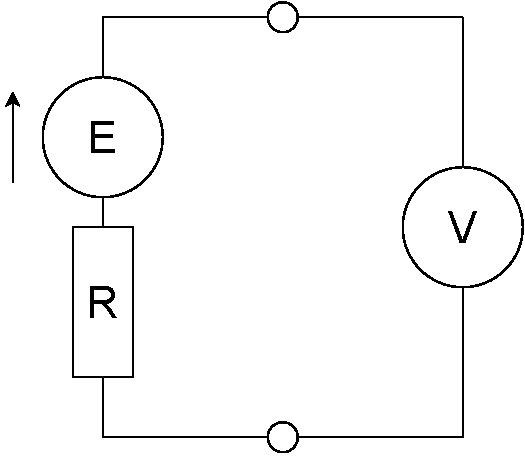
\includegraphics[width=5cm]{schematics/analog_voltage.pdf}
	\caption{Voltage measurement schematic}
	\label{fig:voltage_schematics}
\end{figure}

\subsubsection*{Analog}

\begin{table}[H]
	\centering
	\begin{tabular}{ c | c | c | c | c | c | c | c}
		$R_c [\unit{\ohm}]$ & $\alpha$ & $\alpha_{max}$  & $V_r [\unit{\volt}]$ & $V [\unit{\volt}]$ & $\Delta V [\unit{\volt}]$ & $\delta V  \unit{\percent}$ & $V \pm \Delta V [\unit{\volt}]$\\
		\hline
		0 & 40 & 75 & 7.5 & 4.0 & 0.0375 & 0.9375 & $4.00 \pm 0.04$\\
		\hline
		10 & 40 & 75 & 7.5 & 4.0 & 0.0375 & 0.9375 & $4.00 \pm 0.04$\\
		\hline
		100 & 39.5 & 75 & 7.5 & 3.95 & 0.0375 & 0.949367 & $3.95 \pm 0.04$\\
		\hline
		1000 & 35 & 75 & 7.5 & 3.5 & 0.0375 & 1.071429 & $3.50 \pm 0.04$\\
		\hline
		5000 & 56 & 75 & 0.15 & 0.112 & 0.00075 & 0.669643 & $0.1120 \pm 0.0008$\\
		\hline
		10000 & 30 & 75 & 0.15 & 0.06 & 0.00075 & 1.25 & $0.0600 \pm 0.0008$
	\end{tabular}
	\caption{Analog voltage measurement for $E \sim \SI{3.9}{\volt}$ ($R_c$ -- circuit resistance, $\alpha$ -- actual needle swing, $\alpha_{max}$ -- maximal swing, $V_r$ -- range, $V$ -- calculated voltage, $\Delta V$ -- absolute error, $\delta V$ -- relative error)}
	\label{tab:analog_volt_1}
\end{table}

\begin{table}[H]
	\centering
	\begin{tabular}{ c | c | c | c | c | c}
		$R_v [\unit{\ohm}]$  & $\Delta_m V [\unit{\volt}]$ & $\delta_m V $ & $c [\unit{\volt}]$ & $V_c [\unit{\volt}]$ & $V_c \pm \Delta V [\unit{\volt}]$\\
		\hline
		7500 & 0 & 0 & 0 & 4 & 4.00 +- 0.04\\
		\hline
		7500 & -0.005(3) & -0.001332 & 0.005(3) & 4.005(3) & $4.01 \pm  0.04$\\
		\hline
		7500 & -0.052(6) & -0.013158 & 0.052(6) & 4.002(6) & $4.01 \pm 0.04$\\
		\hline
		7500 & -0.4(6) & -0.117647 & 0.4(6) & 3.9(6) & $3.97 \pm 0.04$\\
		\hline
		150 & -3.7(3) & -0.970874 & 3.7(3) & 3.845(3) & $3.8453 \pm 0.0008$\\
		\hline
		150 & -4 & -0.985222 & 4 & 4.06 & $4.0600 \pm 0.0008$
	\end{tabular}
	\caption{Analog voltage measurement for $E \sim \SI{3.9}{\volt}$ ($R_v$ -- internal voltmeter resistance, $\Delta_m V$ -- systematic error, $\delta_m V$ -- ?, $c$ -- correction factor, $V_c$ -- ?}
	\label{tab:analog_volt_2}
\end{table}

Example calculations for $R_c = \SI{100}{\ohm} $ are shown in Equations~\ref{eq:analog_V},~\ref{eq:analog_Delta_V},~\ref{eq:analog_delta_V},~\ref{eq:analog_R_v},~\ref{eq:analog_Delta_m},~\ref{eq:analog_delta_m},~\ref{eq:analog_c},~\ref{eq:analog_V_c}.

\begin{equation}
	 V = \frac{\alpha\cdot V_{r}}{\alpha_{max}} = \frac{39.5\cdot \SI{7.5}{\volt}}{75} = \SI{3.95}{\volt}
	 \label{eq:analog_V}
\end{equation}

\begin{equation}
	\Delta V = \frac{V_{r}\cdot cl}{100\unit{\percent}} = \frac{\SI{7.5}{\volt}\cdot 0.5\unit{\percent}}{100 \unit{\percent}} = \SI{0.0375}{\volt}
	\label{eq:analog_Delta_V}
\end{equation}

\begin{equation}
	  \delta V = \frac{\Delta V}{V}\cdot 100\unit{\percent} = \frac{0.0375}{3.95}\cdot 100\unit{\percent} \approx 0.949367\unit{\percent}
	  \label{eq:analog_delta_V}
\end{equation}

\begin{equation}
	R_v = V_r\cdot \SI{1}{\frac{\kilo\ohm}{\volt}} = \SI{7.5}{\volt}\cdot \SI{1000}{\frac{\ohm}{\volt}} = \SI{7500}{\ohm}
	\label{eq:analog_R_v}
\end{equation}

\begin{equation}
	\Delta_m V = -V\cdot\frac{R_c}{R_v} = -\SI{3.95}{\volt}\cdot\frac{\SI{100}{\ohm}}{\SI{7500}{\ohm}} = -\SI{0.052(6)}{\volt}
	\label{eq:analog_Delta_m}
\end{equation}

\begin{equation}
	\delta_m V = -\frac{R_c}{R_c + R_v} = -\frac{\SI{100}{\ohm}}{\SI{100}{\ohm} + \SI{7500}{\ohm}} \approx -0.013158
	\label{eq:analog_delta_m}
\end{equation}

\begin{equation}
	c = -\Delta_m V = -\SI{0.052(6)}{\volt} = \SI{0.052(6)}{\volt}
	\label{eq:analog_c}
\end{equation}

\begin{equation}
	V_c = V + c = \SI{3.95}{\volt} + \SI{0.052(6)}{\volt} = \SI{4.002(6)}{\volt}
	\label{eq:analog_V_c}
\end{equation}


\subsubsection*{Digital}

\begin{table}[H]
	\centering
	\begin{tabular}{ c | c |  c | c | c | c | c}
		$R_c [\unit{\ohm}]$  & Accuracy & $V_r [\unit{\volt}]$ & $V [\unit{\volt}]$ & $\Delta V [\unit{\volt}]$ & $\delta V [\unit{\percent}]$ & $V \pm \Delta V [\unit{\volt}]$ \\
	\end{tabular}
	\caption{Digital voltage measurement for $E \sim \SI{3.9}{\volt}$ ($R_c$ -- circuit resistance, Accuracy: $\pm$ (a$\unit{\percent}$ of reading + b$\unit{\percent}$ of range), $V_r$ -- range, $V$ -- measured voltage, $\Delta V$ -- absolute error, $\delta V$ -- relative error)}
	\label{tab:digital_voltage_1}
\end{table}

\begin{table}[H]
	\centering
	\begin{tabular}{  c | c | c | c | c | c}
	 $R_v [\unit{\ohm}]$ & $\Delta_m V [\unit{\volt}]$ & $\delta_m V$ & $c [\unit{\volt}]$ & $V_c [\unit{\volt}]$ & $V_c \pm \Delta V [\unit{\volt}]$\\
	\end{tabular}
	\caption{Digital voltage measurement for $E \sim \SI{3.9}{\volt}$ ($R_v$ -- internal voltmeter resistance, $\Delta_m V$ -- systematic error, $\delta_m V$ -- ?, $c$ -- correction factor, $V_c$ -- ?}
	\label{tab:digital_voltage_2}
\end{table}

\subsection{Voltage divider}